% ============================================================
% PROTOTYPE OVERVIEW -- Team 0109D (StepUp) -- ESC204 Winter 2026
% ============================================================
\documentclass[12pt, letterpaper]{article}
\usepackage[margin=0.5in]{geometry}
\usepackage[T1]{fontenc}
\usepackage[scaled=1]{helvet}
\renewcommand{\familydefault}{\sfdefault}
\usepackage[utf8]{inputenc}
\usepackage{graphicx}
\usepackage{booktabs}
\usepackage{tabularx}
\usepackage{float}
\usepackage{caption}
\usepackage{hyperref}
\usepackage{amsmath}
\usepackage{enumitem}
\usepackage{xcolor}
\usepackage{titlesec}
\usepackage{multicol}

\titleformat{\section}{\large\bfseries}{\thesection}{0.6em}{}
\titleformat{\subsection}{\normalsize\bfseries}{\thesubsection}{0.5em}{}
\titleformat{\subsubsection}[runin]{\normalsize\bfseries}{}{0em}{}[.]
\titlespacing*{\section}{0pt}{6pt}{2pt}
\titlespacing*{\subsection}{0pt}{4pt}{1pt}
\titlespacing*{\subsubsection}{0pt}{3pt}{3pt}
\setlist{nosep, leftmargin=1.2em, itemsep=1pt, parsep=0pt}
\captionsetup{font=small, skip=2pt, labelfont=bf}
\hypersetup{colorlinks=true, linkcolor=blue!70!black, urlcolor=blue!60!black}
\graphicspath{{images/}}
\setlength{\parskip}{2pt plus 1pt minus 1pt}
\setlength{\parindent}{0pt}
\setlength{\floatsep}{3pt plus 1pt minus 1pt}
\setlength{\textfloatsep}{3pt plus 1pt minus 1pt}
\setlength{\intextsep}{3pt plus 1pt minus 1pt}
\setlength{\abovecaptionskip}{2pt}
\setlength{\belowcaptionskip}{0pt}

\begin{document}

\begin{center}
    {\LARGE\textbf{Prototype Overview}}\\[2pt]
    {\normalsize Team 0109D (StepUp) \quad$\vert$\quad ESC204 \quad$\vert$\quad Winter 2026}
\end{center}
\vspace{-2pt}\noindent\rule{\textwidth}{0.6pt}\vspace{3pt}

% ============================================================
% 1  INTRODUCTION + AS-BUILT
% ============================================================
\section{Introduction and System Description}

Our prototype is an \textbf{automated, motor-driven ridge track with a dual-sided air nozzle carriage} that verifies the clearing mechanism of our Design Concept: translating a high-velocity planar air blade along a roof ridge to dislodge wet debris without physical contact. It was built collaboratively: Memo led fluid dynamics testing; Markiyan built the firmware and stepper logic; Kimmy developed the specification and verification protocols; Rihanna led all CAD, 3D print submissions, and the engineering notebook; Hannah coordinated procurement and test hosting; and Karys contributed CAD, documentation, and verification.

\begin{figure}[H]
\centering
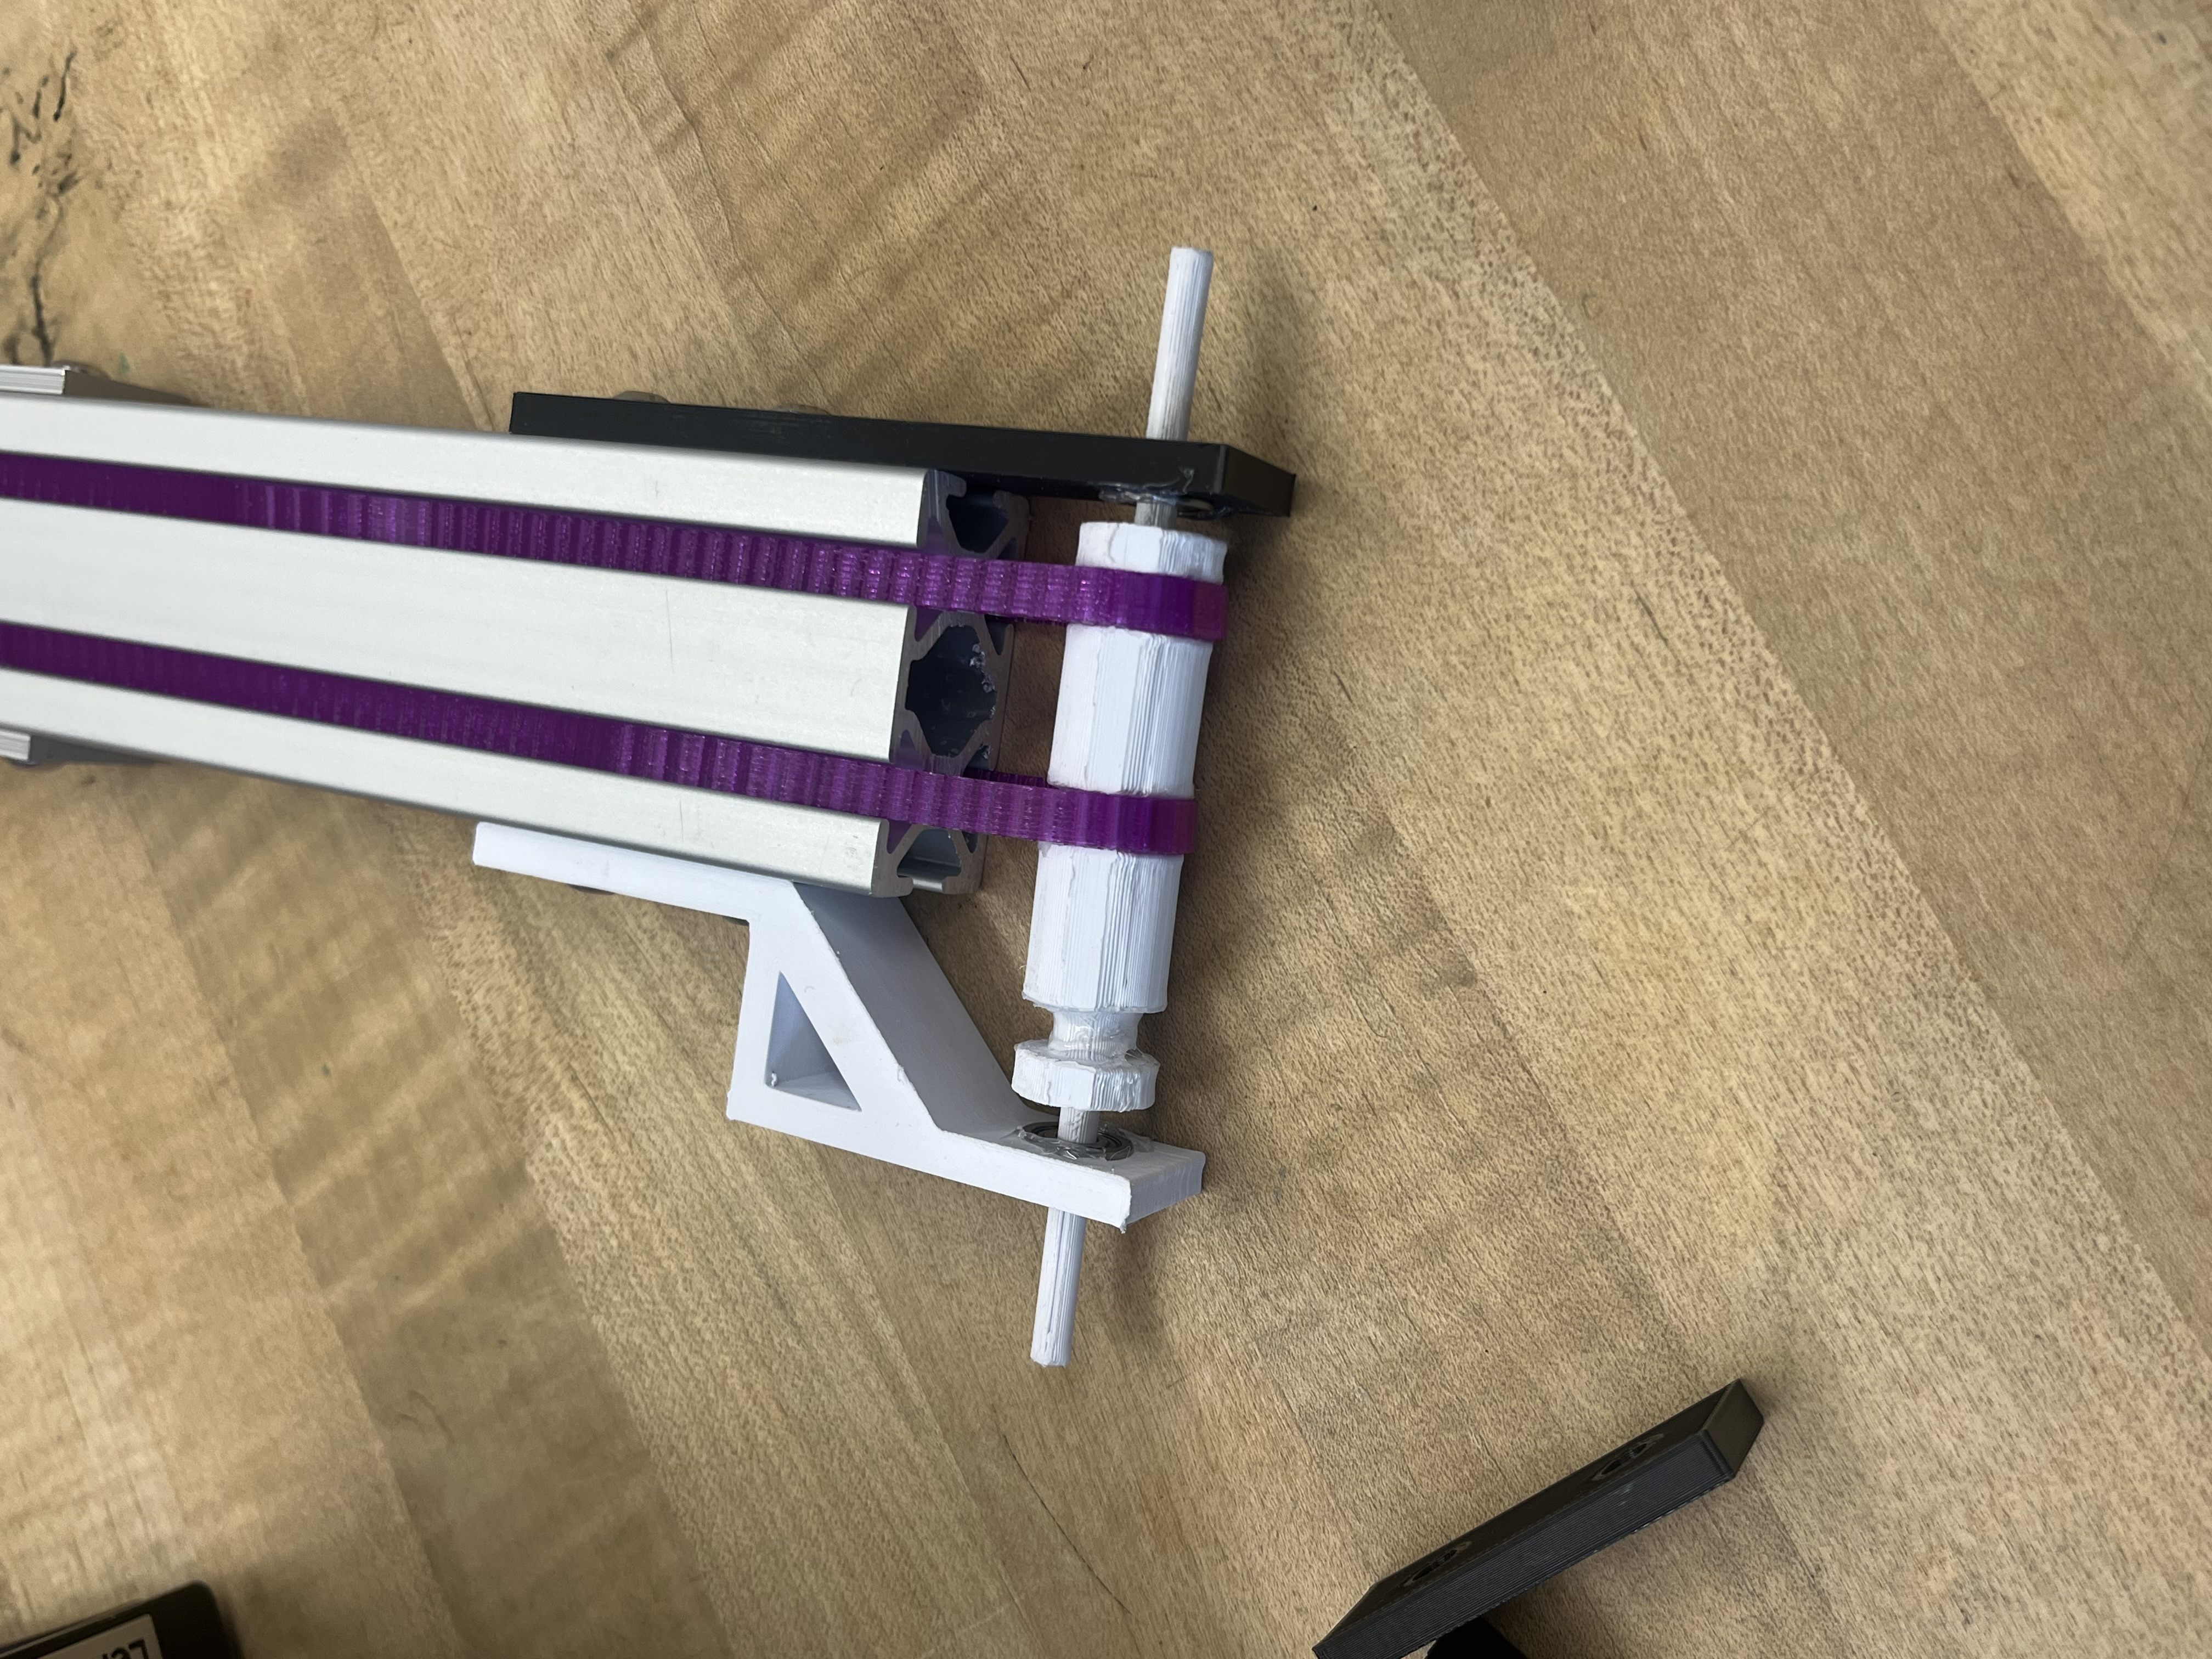
\includegraphics[width=0.55\textwidth]{V2RidgeTrackSystem.jpeg}
\caption{As-built prototype (V2): 60\,cm aluminum T-slot track, V2 pulleys with indented TPU belt, Nema\,17 stepper, nozzle carriage, and D2FS-FL-N limit switches at each end. \href{https://drive.google.com/drive/folders/1wNK_jYUvHXoMne_cIdYbAIURdvYpuG-J}{\textit{[Track overview video]}}}
\label{fig:asbuilt}
\end{figure}

\vspace{-4pt}
The system has two functional halves: \textbf{(1) Translation} (Nema\,17 stepper + A4988 driver + GT2 belt + Pico with limit-switch reversal, traversing a 60\,cm track) and \textbf{(2) Clearing} (Dyson hair dryer through a custom converging slit nozzle at 30$^\circ$, producing a planar shear layer; see \texttt{Air\_Source\_Abstraction\_Justification.pdf} in \texttt{04.4} for the Dyson abstraction rationale). The architecture maps directly to our Phase\,2 subsystems (Electrical, Mechanical, Software); full mapping table in \href{https://github.com/memo-ozdincer/ESC203-AI-Prototypes/blob/master/dossier_artifacts/PraxisCode.py}{\texttt{PraxisCode.py}} and the \texttt{Specification.xlsx} in \texttt{04\_Prototype}.

% ============================================================
% 2  TRACK & PULLEY ITERATIONS
% ============================================================
\section{Track \& Pulley System Iterations}

The mechanical drivetrain went through two major versions. Hannah submitted all MYFab orders; Rihanna led the CAD redesigns. Full iteration photos (red/blue border comparisons) and the \textit{List of Changes During Integration} document are in \texttt{04.3\_Integration}.

\begin{figure}[H]
\centering
\begin{minipage}[t]{0.48\textwidth}
    \centering
    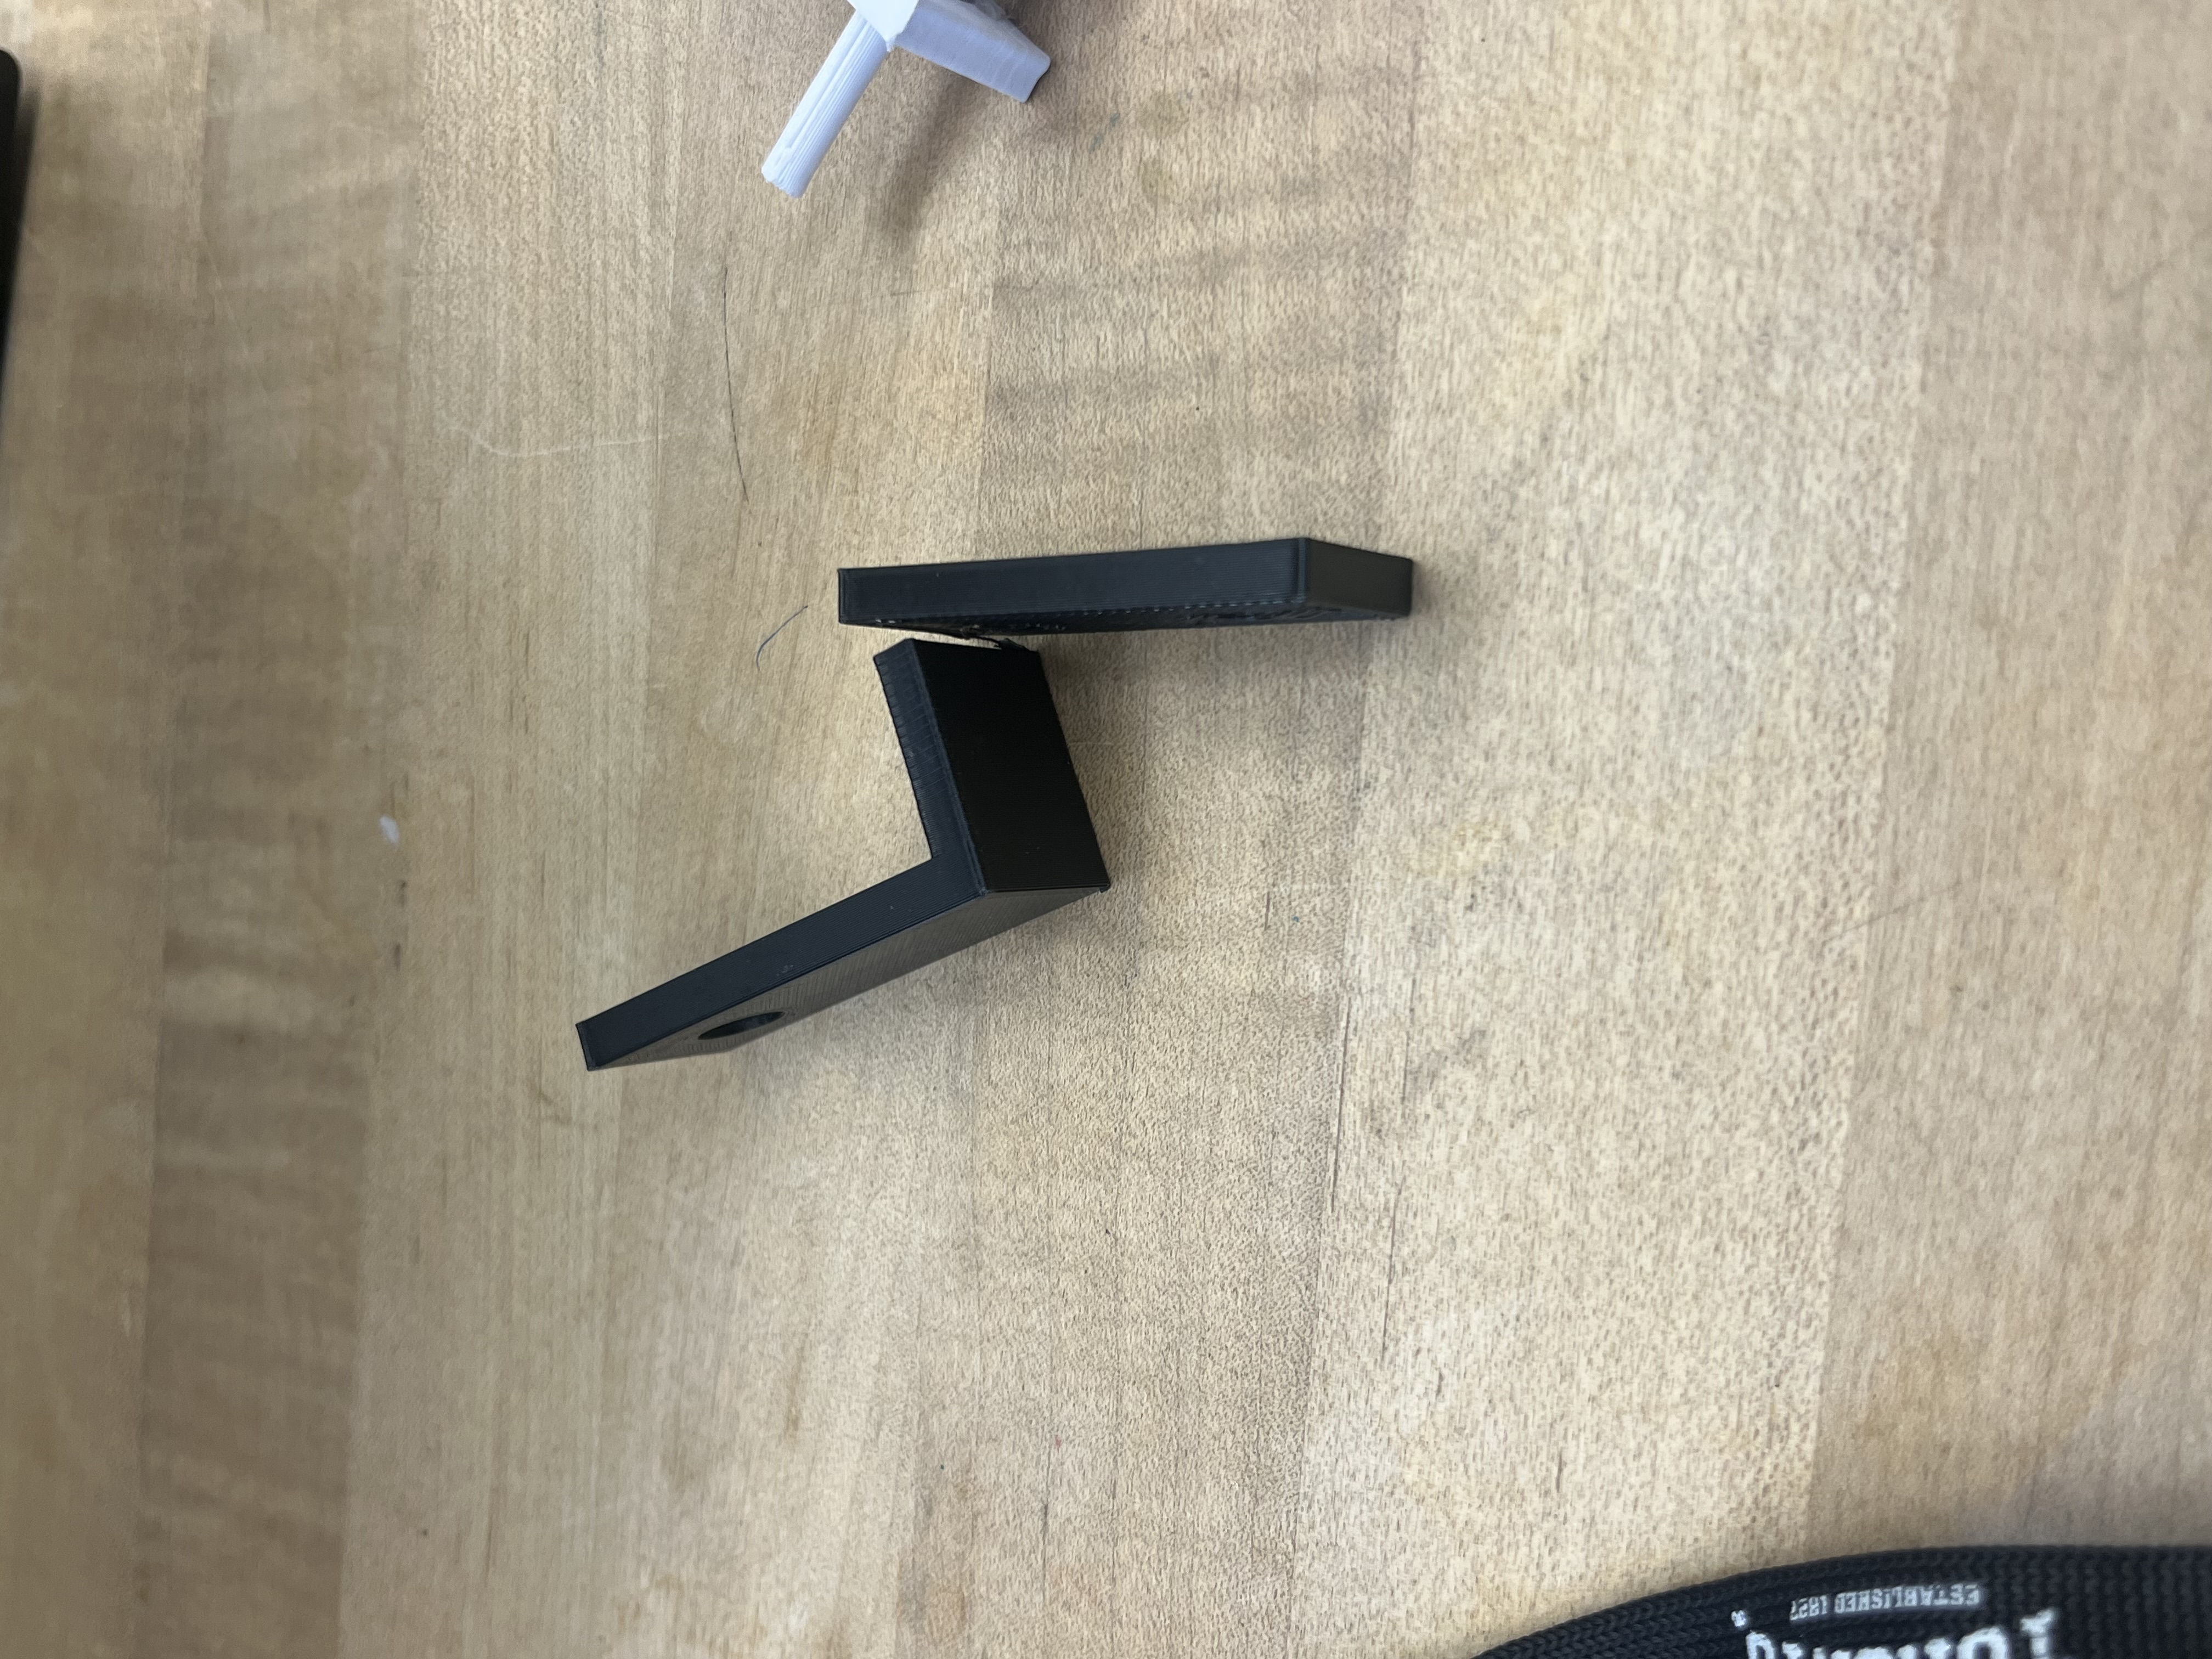
\includegraphics[width=\textwidth, height=4.2cm, keepaspectratio]{V1BrokenPulleyAxle.jpeg}
    \caption{V1 failure: axle bent under belt tension. FDM printed a teardrop cross-section instead of circular; sanding helped but the thin geometry could not hold. L-bracket corners also deformed. \textit{Photo:} \texttt{04.3}.}
    \label{fig:v1axle}
\end{minipage}\hfill
\begin{minipage}[t]{0.48\textwidth}
    \centering
    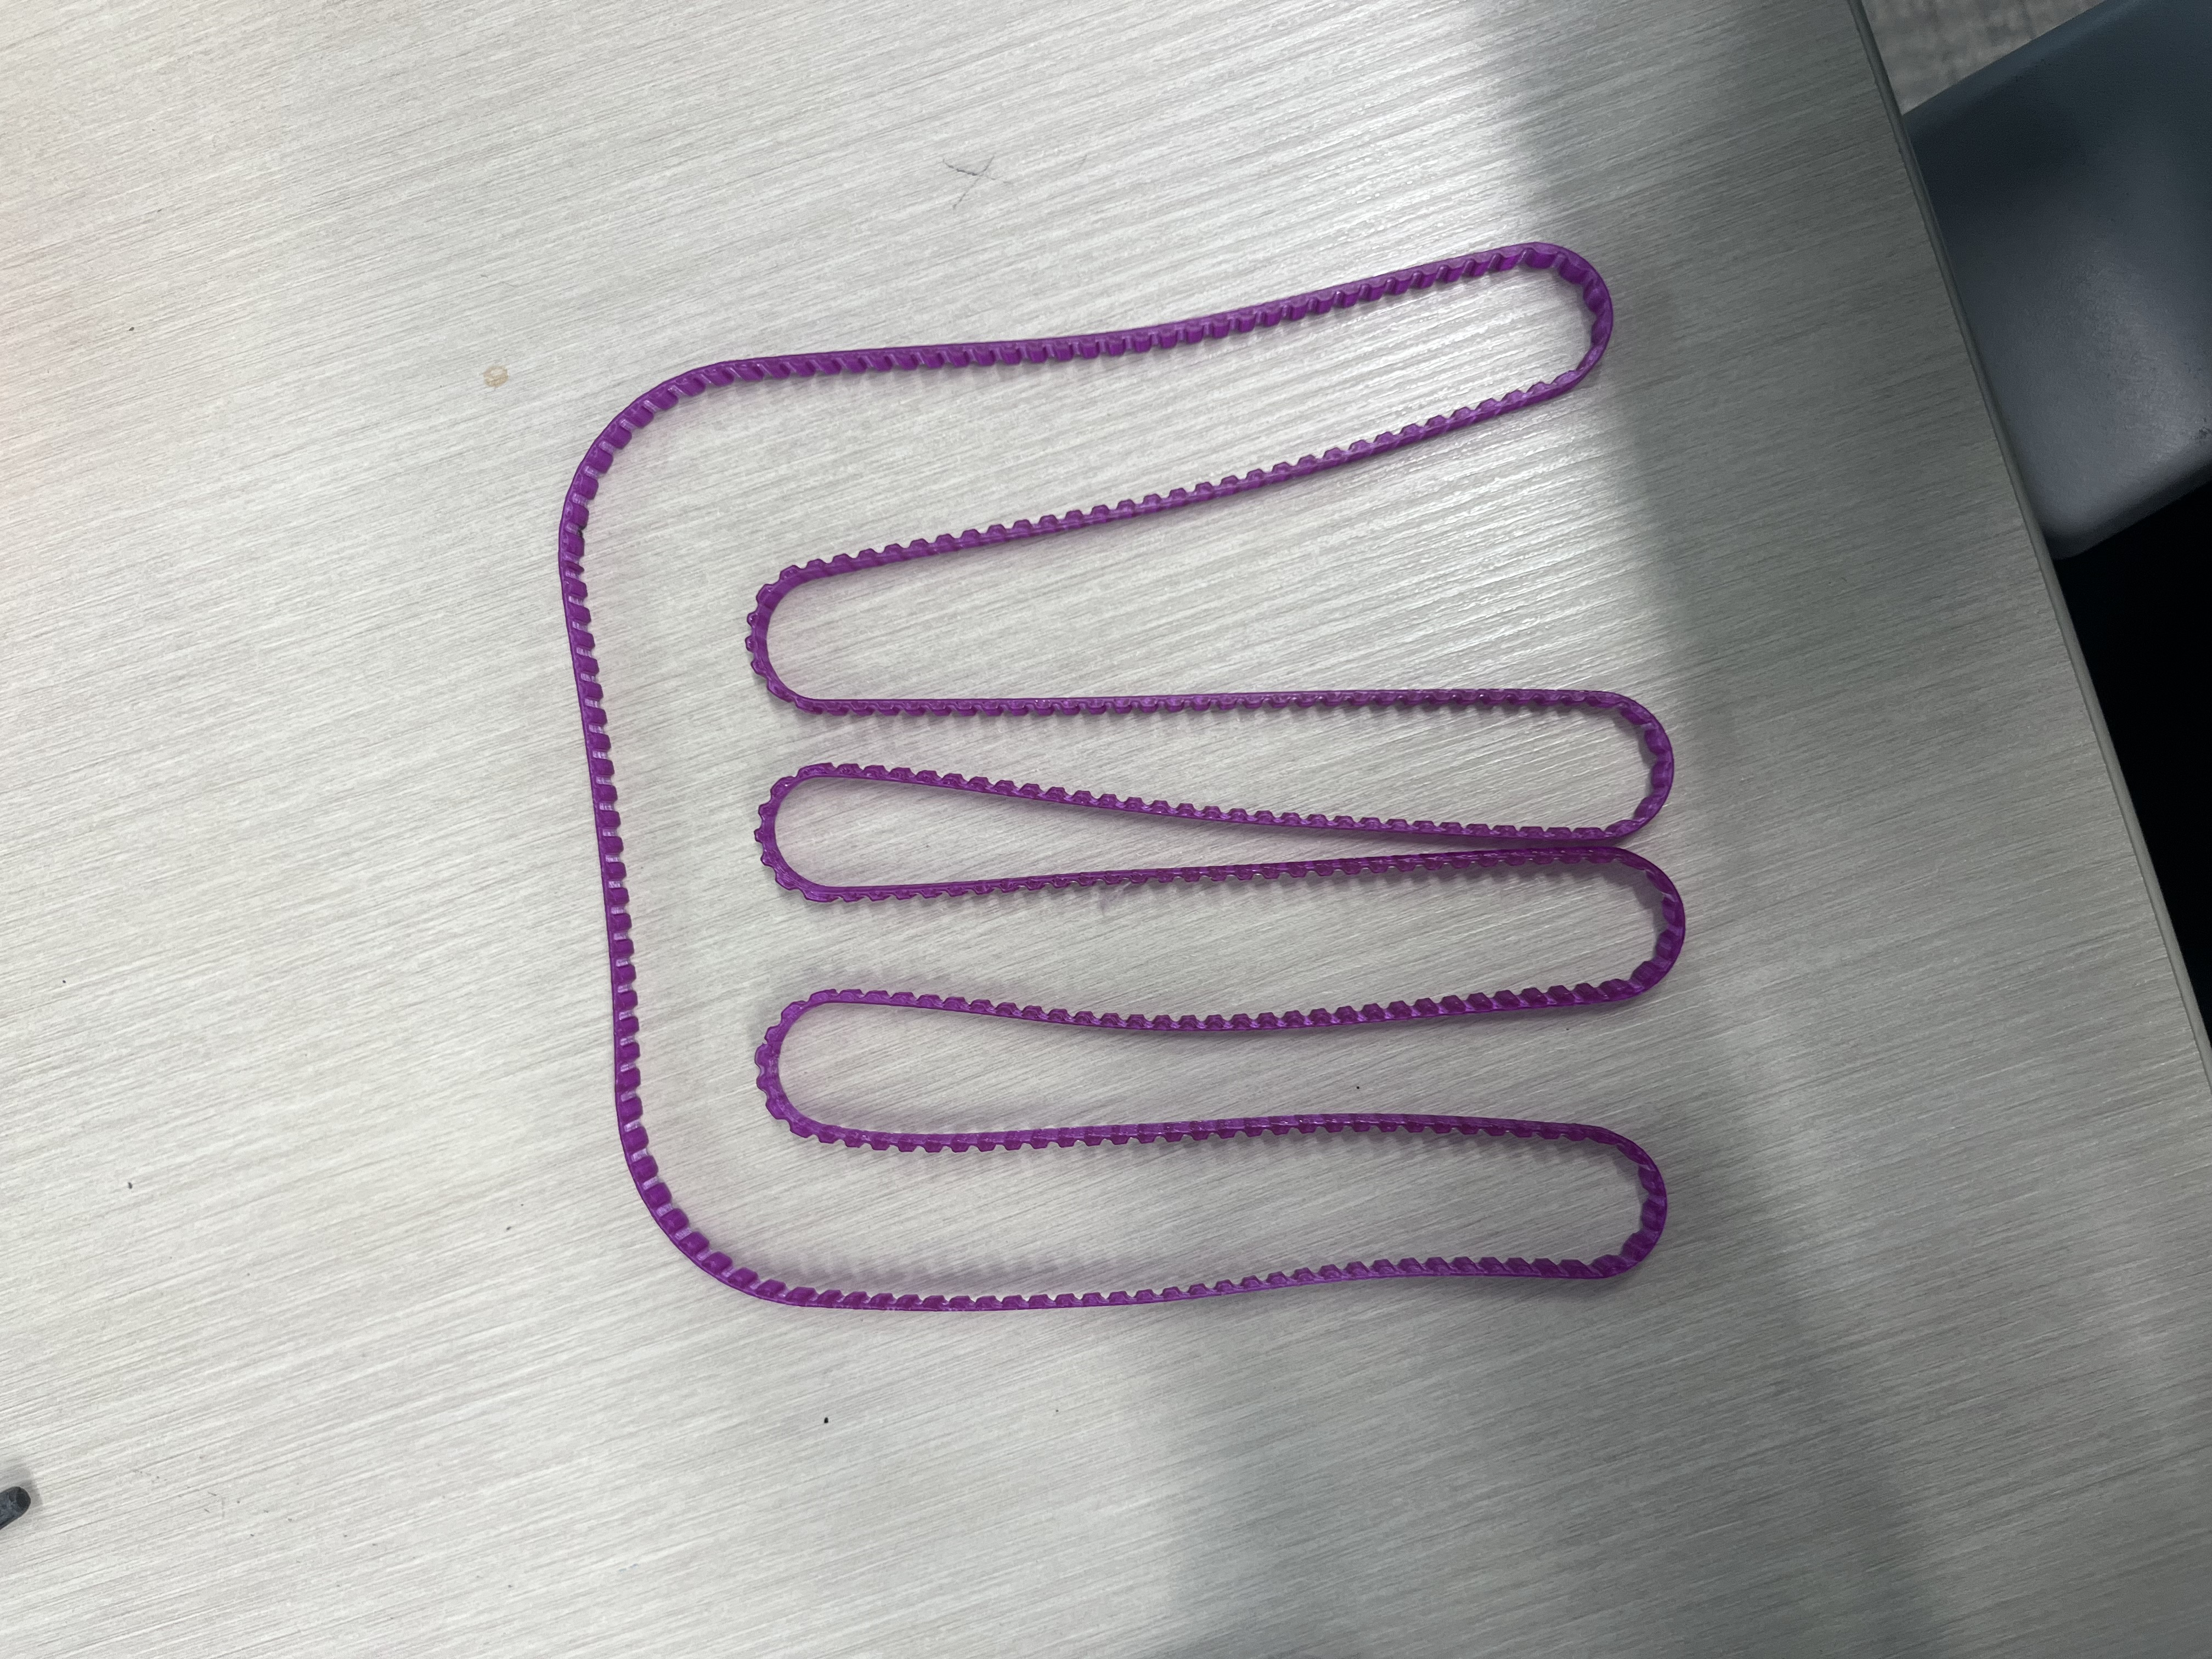
\includegraphics[width=\textwidth, height=4.2cm, keepaspectratio]{BeltWithIndentations.jpeg}
    \caption{V2 TPU belt with CAD-designed grip indents (visible ridges). V1 belt was smooth and slipped on pulleys; hot glue also failed on TPU. Compare with \texttt{OldTimingBelt.png} and \texttt{V1vsV2PulleyAxle} in \texttt{04.3}.}
    \label{fig:v2belt}
\end{minipage}
\end{figure}

\vspace{-4pt}
\begin{table}[H]
\centering\small
\caption{Full mechanical iteration history. Photos and videos of each version in \texttt{04.2\_Build/Mechanical} and \texttt{04.3\_Integration}. Videos: \href{https://drive.google.com/drive/folders/1wNK_jYUvHXoMne_cIdYbAIURdvYpuG-J}{\textit{TensionInAxlePulley.mov}}, \href{https://drive.google.com/drive/folders/1wNK_jYUvHXoMne_cIdYbAIURdvYpuG-J}{\textit{V2RidgeTrackMovement.MOV}}.}
\label{tab:mech}
\begin{tabularx}{\textwidth}{@{}l X X@{}}
\toprule
\textbf{Component} & \textbf{V1 (Failed)} & \textbf{V2 (Final)} \\
\midrule
Track  & 40\,cm (2$\times$20\,cm extrusions, Mar\,11). Too short for meaningful travel. & 60\,cm (3$\times$20\,cm, Order \#3 Mar\,19). 56\,cm active between switches. \\
Axles  & Thin; teardrop FDM artifact (Fig.\,\ref{fig:v1axle}). Bent under tension. & Thicker center; true circular. Confirmed with MYFab mentor Mar\,10. \\
Brackets & L-shaped corners deformed under belt load. & Triangle-reinforced gussets; rigid under load. \\
Belt   & Smooth TPU slipped on pulleys. Hot glue failed on TPU. & Indented TPU with grip teeth (Fig.\,\ref{fig:v2belt}). GT2 pitch, 20-tooth. \\
\bottomrule
\end{tabularx}
\end{table}

% ============================================================
% 3  NOZZLE ITERATIONS
% ============================================================
\section{Nozzle Design Evolution}

The nozzle is the core of the clearing subsystem. Rihanna designed the custom air blade geometry in SolidWorks; the 30$^\circ$ angle of attack was justified by vector decomposition of the airflow into normal ($F_y$) and tangential ($F_x$) components. STL files for all nozzle versions are in \texttt{04.2\_Build/Mechanical/3D Print Files}.

The Design Concept originally planned a ball pump as the air source, but early testing showed it only produces pulsed, low-volume bursts, which cannot sustain the boundary-layer shear needed for clearing. The team pivoted to a Dyson hair dryer for continuous high-CFM flow. With a reliable air source established, the design variable became the \textbf{nozzle exit geometry}: the question was whether reshaping the circular Dyson output into a narrow planar slit would improve clearing.

The prototype nozzle is a converging channel that compresses the circular airflow into a thin, wide slit. This produces a high-velocity planar shear layer (an ``air blade'') rather than a localized impact column. The carriage mount holds this nozzle at a fixed 30$^\circ$ relative to the roof surface. At 30$^\circ$, the $F_y$ component provides enough downward pressure for Coanda-effect boundary attachment (the air ``sticks'' to the surface and gets under debris) without being so steep that it pins debris down. The $F_x$ component is maximized to sweep dislodged material down the slope. Angles above 45$^\circ$ pin debris via static friction; below 15$^\circ$, airflow deflects over the debris entirely.

The physical nozzle cart is dual-sided, meaning it has slit exits on both sides of the carriage, enabling clearing on both the forward and reverse pass. Nozzle CAD design decisions are documented in \texttt{04.2\_Build/Mechanical/Air Nozzle + Cart CAD design decision.docx}; V1 and V2 STL files in the \texttt{3D Print Files} subfolder.

% ============================================================
% 4  ELECTRICAL & FIRMWARE ITERATIONS
% ============================================================
\section{Electrical \& Firmware Iterations}

The electrical subsystem iterated three times (Markiyan led). Each version was abandoned after a specific failure.

\begin{figure}[H]
\centering
\begin{minipage}[t]{0.48\textwidth}
    \centering
    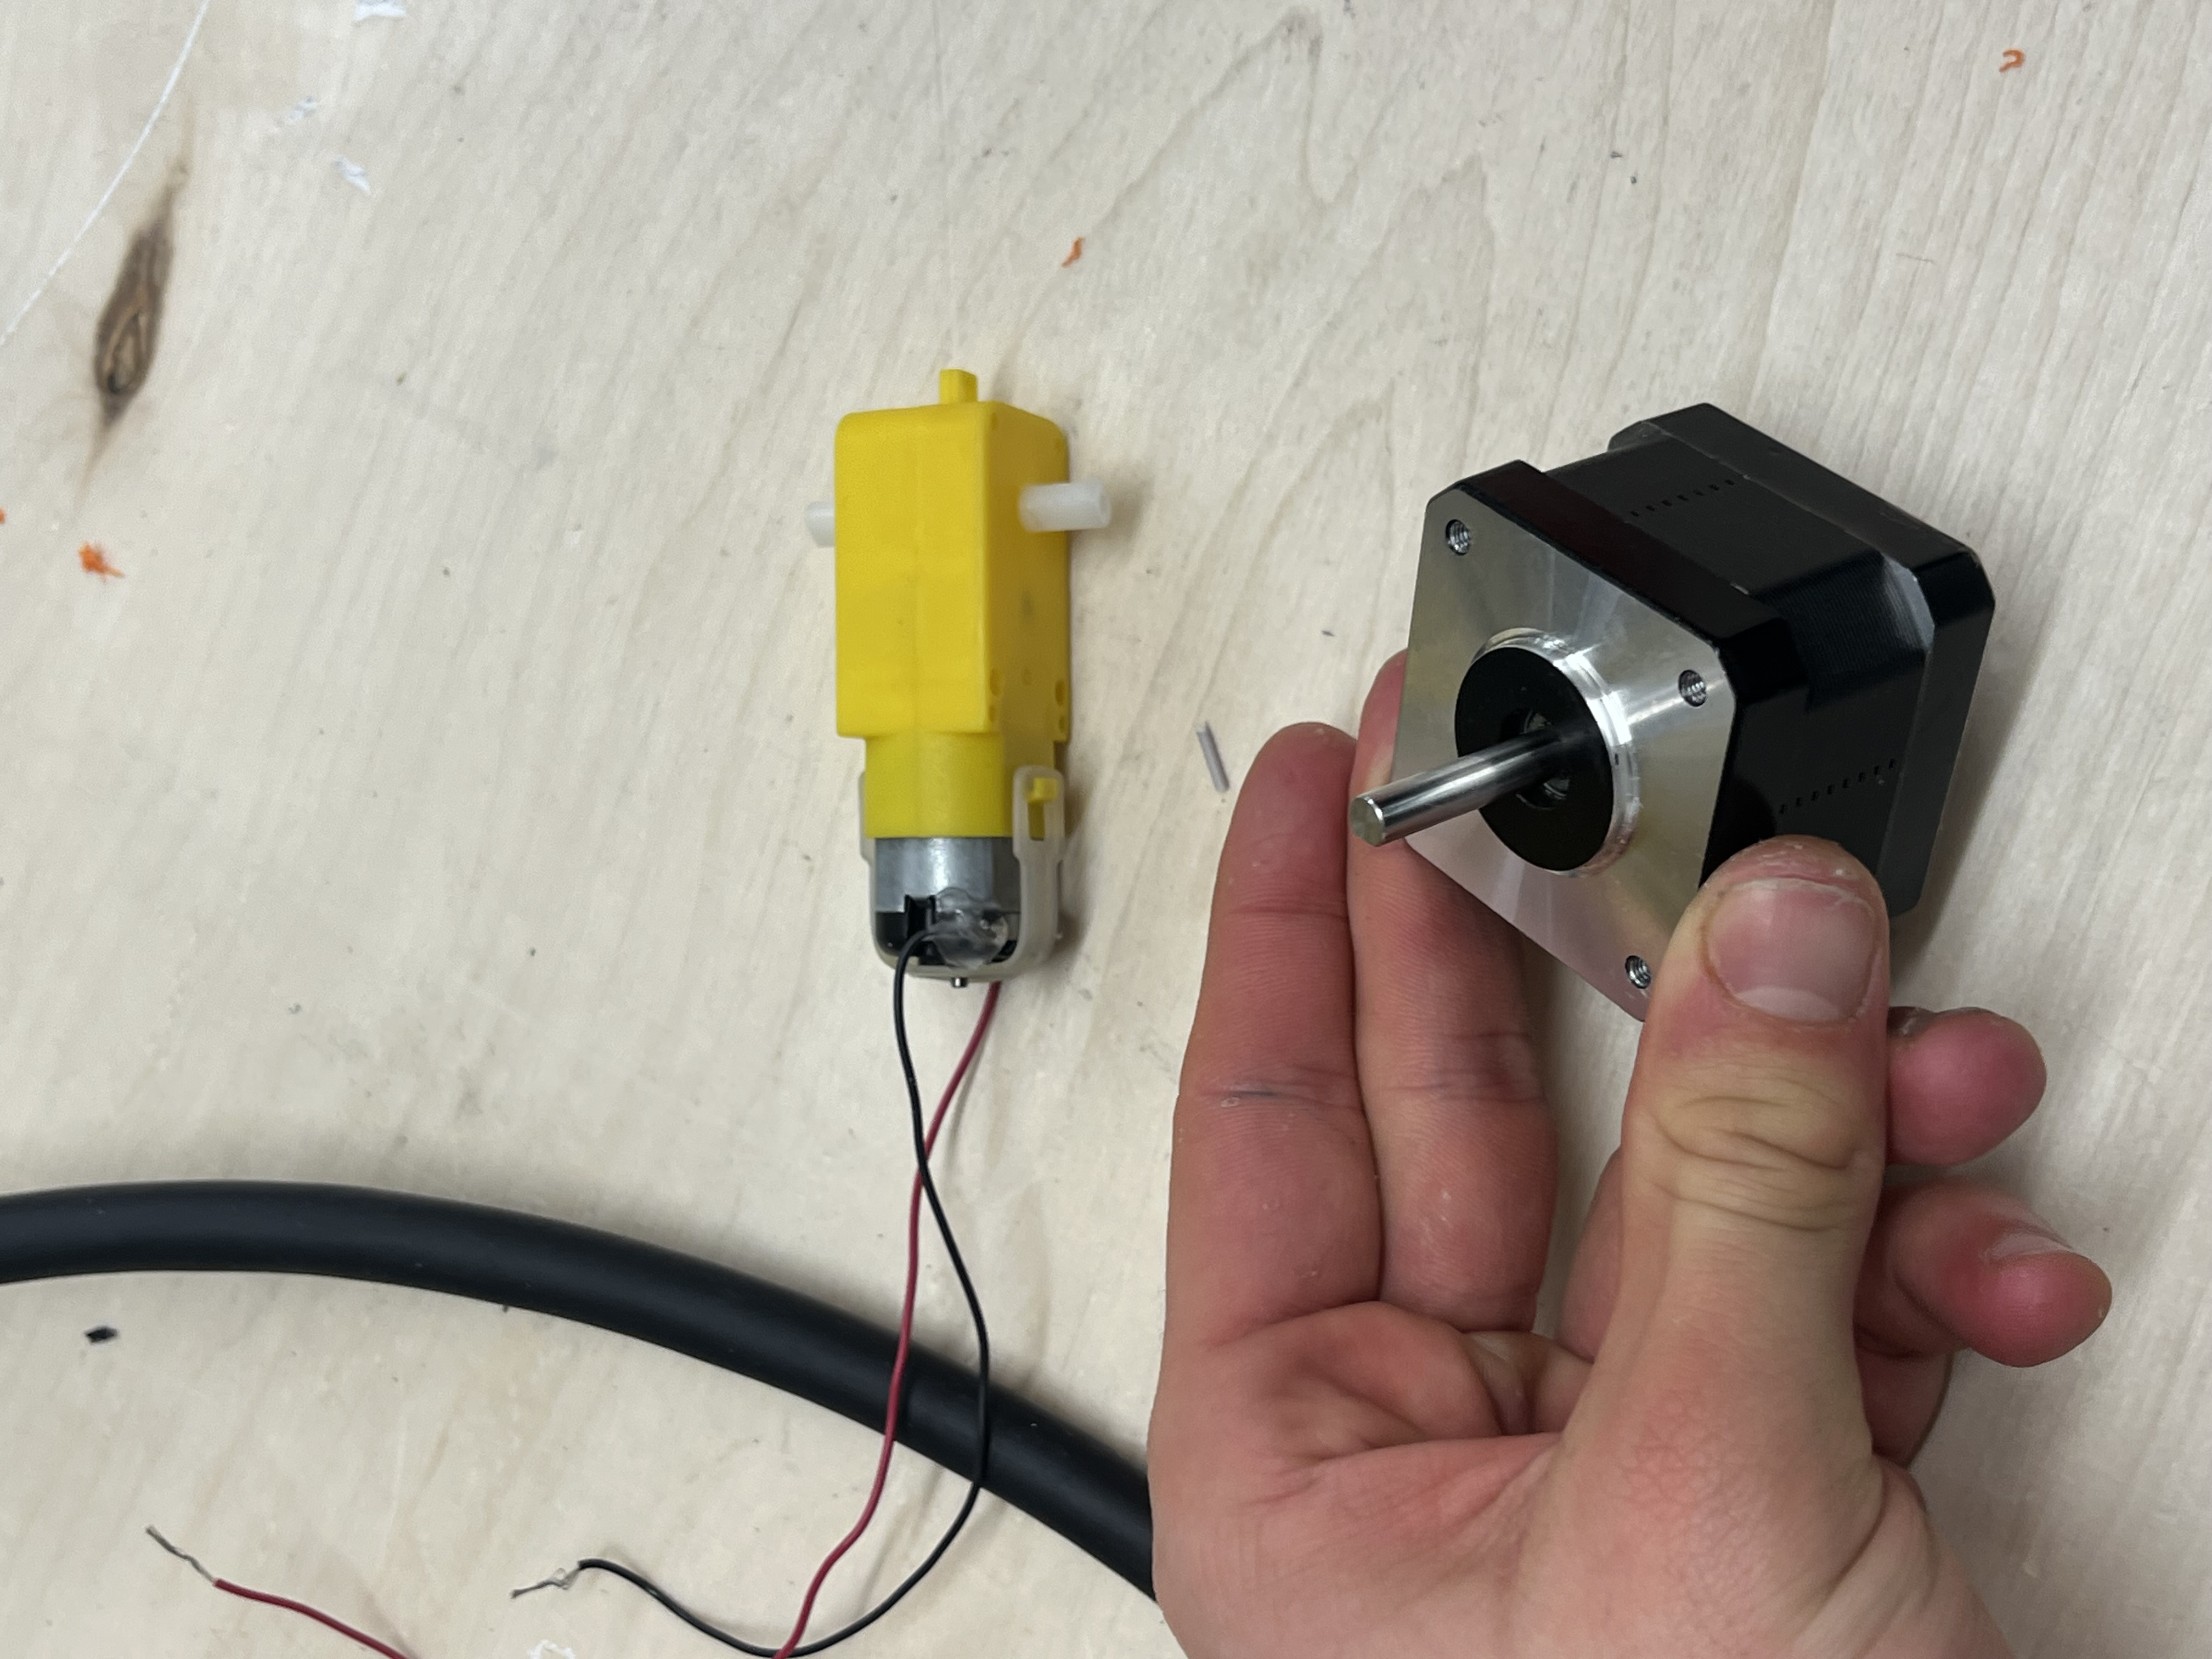
\includegraphics[width=\textwidth, height=4.2cm, keepaspectratio]{HBridge_Motor_Iteration2.jpeg}
    \caption{Motor swap: original 3--6\,V DC gearmotor (yellow) vs.\ final Nema\,17 stepper. DC motor had no positional accuracy under variable load. \href{https://drive.google.com/drive/folders/1wNK_jYUvHXoMne_cIdYbAIURdvYpuG-J}{\textit{[Jitter failure video]}}}
    \label{fig:motor}
\end{minipage}\hfill
\begin{minipage}[t]{0.48\textwidth}
    \centering
    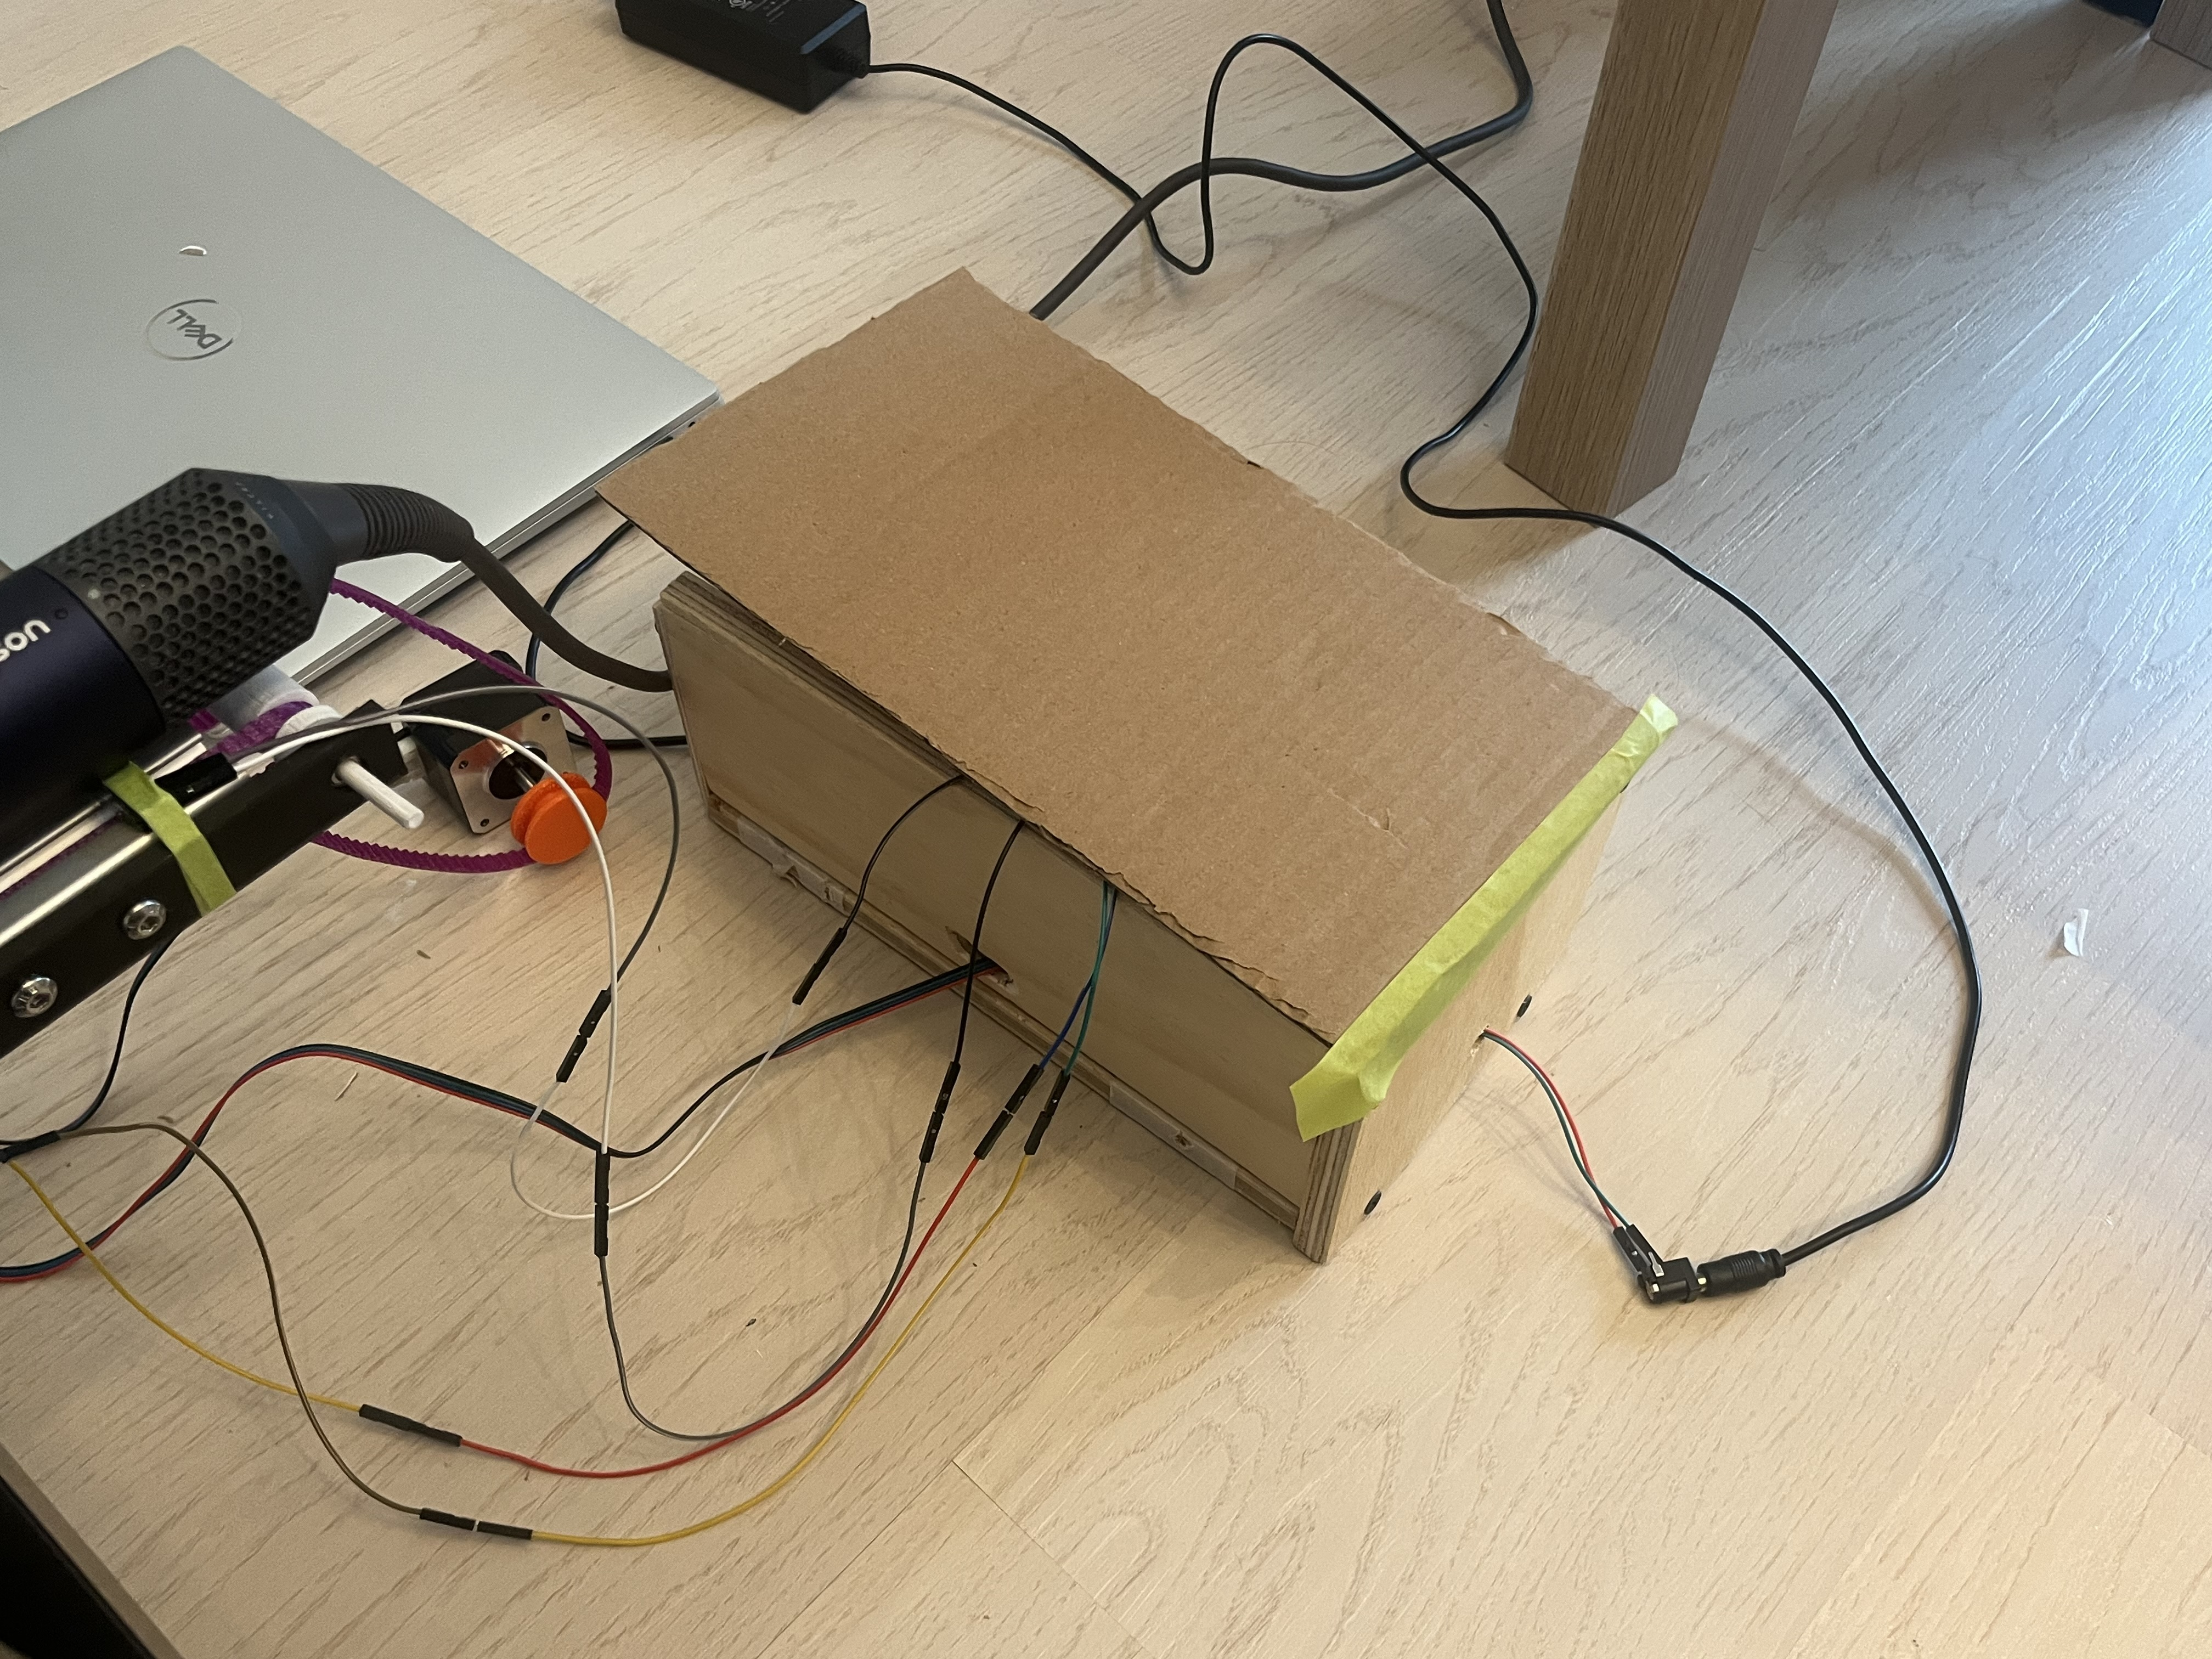
\includegraphics[width=\textwidth, height=4.2cm, keepaspectratio]{ClosureElectrical.jpeg}
    \caption{Final enclosure: A4988 driver, Pico, screw-terminal power blocks with isolated 5\,V/12\,V rails. All iterations documented in \texttt{04.2\_Build/Electronics/Design Process of electronics.docx}.}
    \label{fig:elec}
\end{minipage}
\end{figure}

\vspace{-4pt}
\begin{table}[H]
\centering\small
\caption{Electrical iteration history. Photos: \texttt{04.2\_Build/Electronics}. Videos: \texttt{04.3\_Integration}.}
\begin{tabularx}{\textwidth}{@{}c l X l@{}}
\toprule
& \textbf{Configuration} & \textbf{Failure / Outcome} & \textbf{Artifact} \\
\midrule
1 & DC motor + breadboard + 9\,V & No dead reckoning; position drifts under load & \texttt{DC\_Motor\_*.jpeg} \\
2 & DC motor + L298N H-Bridge & Voltage drop $\rightarrow$ stall and jitter & \href{https://drive.google.com/drive/folders/1wNK_jYUvHXoMne_cIdYbAIURdvYpuG-J}{\textit{Jitter video}} \\
3 & Nema\,17 + A4988 + screw terminals & 0.2\,mm/step precision, no jitter & Fig.\,\ref{fig:elec} \\
\bottomrule
\end{tabularx}
\end{table}

\vspace{-4pt}
\textbf{Power segregation:} Shared power rail caused Pico brownouts. Fixed by isolating 5\,V USB logic from 12\,V motor adapter. \textbf{Thermal tuning:} A4988 $V_{REF}$ tuned to ${\sim}$50\% to prevent thermal shutdown. \textbf{Firmware:} Polling of limit switches on GP15/GP16 (pull-up); instant DIR reversal when triggered; 4-cycle auto-stop after 2 round trips. \textbf{Deadzone fix:} Switches take ${\sim}$2\,cm per end, so nozzle overhangs 2\,cm each side for 100\% coverage. Source: \href{https://github.com/memo-ozdincer/ESC203-AI-Prototypes/blob/master/dossier_artifacts/PraxisCode.py}{\texttt{PraxisCode.py}} in \texttt{04.2\_Build/Software}.

% ============================================================
% 5  VERIFICATION: THE THREE-TEST CHAIN
% ============================================================
\section{Verification: Force $\rightarrow$ Geometry $\rightarrow$ Wet Stiction}

We designed a structured three-test verification chain, each building on the previous. All raw data and protocols are in the \texttt{Verification Protocol+Results.xlsx} spreadsheet in \texttt{04.4}. All 8 nozzle test videos: \href{https://drive.google.com/drive/folders/1RAJA95EF-XjMrkhjWkuoIBbONH_DbRVu}{\textit{[Google Drive: circular\_vs\_nozzle]}}.

\subsection{Test 1: Do we have enough force? (Magnitude)}

We taped a rigid cardboard target to a digital kitchen scale and blew the Dyson at it from 4, 8, 12, and 16\,cm across three nozzle geometries. This establishes the raw force baseline before any geometry optimization.

\vspace{-2pt}
\begin{table}[H]
\centering\small
\caption{Measured force (N). All geometries conserve $\sim$1.96\,N within 12\,cm.}
\label{tab:force}
\begin{tabular}{@{}lcccc@{}}
\toprule
\textbf{Nozzle} & \textbf{4\,cm} & \textbf{8\,cm} & \textbf{12\,cm} & \textbf{16\,cm} \\
\midrule
Pure Dyson (Baseline)   & 1.96 & 1.95 & 1.95 & 1.76 \\
Dyson OEM Air Blade     & 1.98 & 1.97 & 1.95 & 1.78 \\
Custom Air Blade (Ours) & 1.96 & 1.95 & 1.93 & 1.72 \\
\bottomrule
\end{tabular}
\end{table}

\vspace{-4pt}
\textbf{Finding:} Total force is conserved across geometries (mass-flow conservation). Reshaping the exit does not create more force; it \textit{redistributes} it into planar shear. Sharp drop at 16\,cm means the nozzle must stay within 12\,cm of the surface. Having confirmed sufficient magnitude, we moved to geometry optimization.

\subsection{Test 2: Which geometry clears better? (Distance \& Angle)}

We built a 30$^\circ$ roof mock-up (35$\times$15\,cm, 40-grit aluminum oxide sandpaper simulating shingles), measured angles with a protractor and alignment frame (axial alignment verified by a second observer), and tested at $d = 10$, 25, and 50\,cm. Three trial sets per configuration. Dry tissue paper simulated loose debris.

\vspace{-2pt}
\begin{table}[H]
\centering\small
\caption{Clearing results. Individual trial videos: \href{https://drive.google.com/drive/folders/1RAJA95EF-XjMrkhjWkuoIBbONH_DbRVu}{\textit{nozzle\_distance1/2/3.mov, circular\_distance1/2/3.mov}}.}
\label{tab:clearing}
\begin{tabularx}{\textwidth}{@{}l X X@{}}
\toprule
\textbf{Dist.} & \textbf{Circular Nozzle} & \textbf{Custom Air Blade} \\
\midrule
10\,cm & Both clear. Geometry negligible at close range. & Both clear. \\
25\,cm & Debris blown lower, shorter distance. & Ejected higher and further. Shear layer penetrates \textit{under} debris. \\
50\,cm & Narrow central path only. Heavy lateral residue from turbulent diffusion. & Full 15\,cm uniform sweep. Coherent planar coverage. \\
\bottomrule
\end{tabularx}
\end{table}

\vspace{-4pt}
At close range both work. At distance, the air blade maintains a coherent wide sweep while the circular nozzle diffuses into a narrow, weak column. Having confirmed geometry matters, we escalated to worst-case conditions.

\subsection{Test 3: Can it clear worst-case wet debris? (Stiction Stress Test)}

Same setup at $d = 50$\,cm, but with \textbf{heavily saturated tissue paper} pressed onto the 40-grit sandpaper. This maximizes stiction and eliminates any aerodynamic profile (see \texttt{Debris\_Model\_Justification.pdf} in \texttt{04.4} for why this is a conservative worst-case analogue).

\begin{itemize}
    \item \textbf{Circular Nozzle (30$^\circ$):} \textcolor{red}{\textbf{FAILED.}} High-pressure column pinned the flat wet tissue \textit{harder} against the surface. Only a few central pieces dislodged.
    \href{https://drive.google.com/file/d/1wO-Wh8iFGygEvBvc3OOH91XQSwhoY_Ws/view}{\textit{[Video: circular\_wet\_test.mov]}}
    \item \textbf{Custom Air Blade (30$^\circ$):} \textcolor{green!50!black}{\textbf{PASSED.}} Planar shear layer slipped beneath the water/sandpaper interface and peeled the saturated debris off.
    \href{https://drive.google.com/file/d/16htpF3ptwKEM5UxYE679x3f3xWmt80h1/view}{\textit{[Video: nozzle\_wet\_test.mov]}}
\end{itemize}

\subsection{Endurance Test (Mechanical)}
Continuous 2-minute cycle, far exceeding the 2-pass spec. Zero stalling; belt held tension through reversals; A4988 within thermal limits. 56\,cm in 22\,s ($v \approx 2.55$\,cm/s). \href{https://drive.google.com/drive/folders/1wNK_jYUvHXoMne_cIdYbAIURdvYpuG-J}{\textit{[Full cycle video; Stopping\_at\_end\_of\_cycle.mp4]}}

% ============================================================
% 6  SPECS
% ============================================================
\section{Performance vs.\ Specification}

\vspace{-2pt}
\begin{table}[H]
\centering\small
\caption{All 11 specs passed. Full protocol: \texttt{VerificationProtocol+Results.xlsx} in \texttt{04.4\_Verification}.}
\label{tab:specs}
\begin{tabularx}{\textwidth}{@{}l X c l@{}}
\toprule
\textbf{Spec ID} & \textbf{Statement} & \textbf{Result} & \textbf{Method} \\
\midrule
O-1.1-ELEC-1 & Traverse track $\geq$2 passes                      & \textcolor{green!50!black}{\textbf{PASS}} & Demo \\
O-2.1-ELEC-1 & No roof access for activation                       & \textcolor{green!50!black}{\textbf{PASS}} & Inspect \\
O-2.2-ELEC-1 & Insulated electrical components                     & \textcolor{green!50!black}{\textbf{PASS}} & Inspect \\
O-3.2-ELEC-1 & Limit switches for direction/energy                 & \textcolor{green!50!black}{\textbf{PASS}} & Demo \\
O-1.1-STRU-1 & Force to dislodge debris                            & \textcolor{green!50!black}{\textbf{PASS}} & Test \\
O-1.1-STRU-2 & Full-width air coverage                             & \textcolor{green!50!black}{\textbf{PASS}} & Test \\
O-4.1-STRU-1 & Low-profile, follows roof contour                   & \textcolor{green!50!black}{\textbf{PASS}} & Inspect \\
O-4.2-STRU-1 & No shingle damage                                   & \textcolor{green!50!black}{\textbf{PASS}} & Inspect \\
O-1.3-SOFT-1 & Autonomous 2-pass CLEARING state                    & \textcolor{green!50!black}{\textbf{PASS}} & Demo \\
O-2.1-SOFT-1 & Ground-level activation                              & \textcolor{green!50!black}{\textbf{PASS}} & Inspect \\
O-3.2-SOFT-1 & OFF state: motors inactive                           & \textcolor{green!50!black}{\textbf{PASS}} & Inspect \\
\bottomrule
\end{tabularx}
\end{table}

% ============================================================
% 7  CHALLENGES + CONTRIBUTION (combined to save space)
% ============================================================
\section{Challenges and Contribution to Design Concept}

Key challenges: (1) Motor stalling/jitter forced a full 3-iteration drivetrain redesign (\href{https://drive.google.com/drive/folders/1wNK_jYUvHXoMne_cIdYbAIURdvYpuG-J}{\textit{video}}). (2) Power brownouts required isolated 5\,V/12\,V rails. (3) FDM teardrop artifacts on V1 axles (Fig.\,\ref{fig:v1axle}) and belt slippage (Fig.\,\ref{fig:v2belt}) required two complete mechanical redesign cycles. (4) A4988 thermal shutdown, resolved by $V_{REF}$ tuning. (5) Limit-switch deadzones compensated by nozzle overhang.

The prototype verified two core hypotheses. \textbf{First}, automated linear translation is feasible: the stepper-driven belt system traverses reliably with mm-precision across 120\,s+ of continuous operation. \textbf{Second}, a planar air blade outperforms a circular nozzle: the three-test chain (Force $\rightarrow$ Angle $\rightarrow$ Wet Stiction) proved that the custom slit nozzle's shear-layer mechanism clears worst-case adhered wet debris where the circular nozzle fails entirely.

Next phase: stepper + isolated power (not DC); planar slit at 30$^\circ$ (Coanda); nozzle within 12\,cm; compressor selection to replace the Dyson abstraction.

\end{document}
